\section*{Решение}
\section{Формулировка краевой задачи}

Введем начало координат в точке А. Отрежем пружину, заменим реакцией:
\begin{figure}[H]
    \begin{center}
        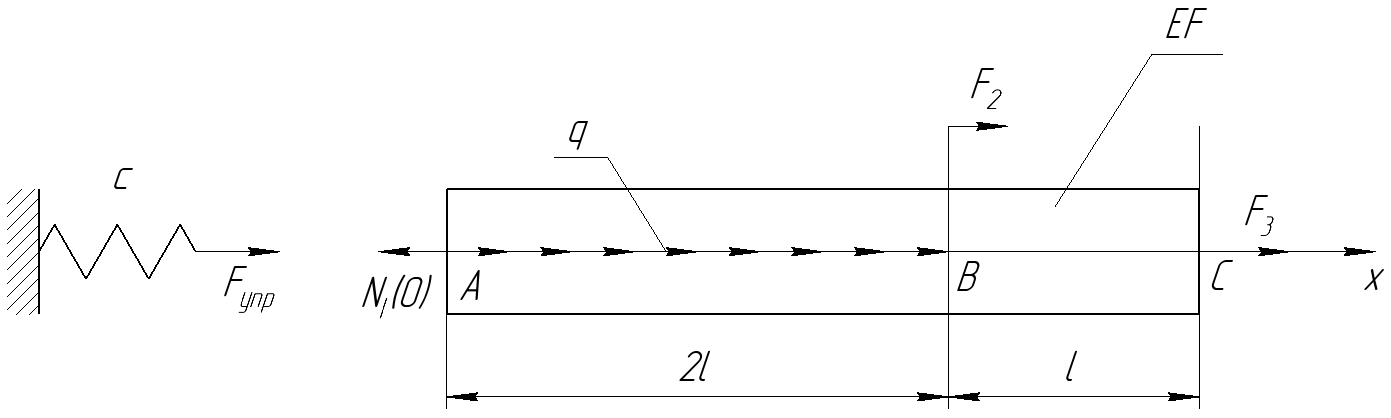
\includegraphics[width = 0.7\linewidth]{pic1.1}
        \caption{Расчетная схема}
        \label{pic1.1}
    \end{center}
\end{figure}

Сила упругости пружины равна:
\begin{equation}
    \label{eq1.1}
    F_{\t{упр}} = c \cdot u(0)
\end{equation}

Разобьем стержень на 2 участка и запишем для них дифференциальное уравнение равновесия:

\begin{enumerate}
    \item Участок $AB$:
    \begin{equation}
        \label{eq1.2}
        EFu_{I}'' (x) + q = 0
    \end{equation}
    \item Участок $BC$:
    \begin{equation}
        \label{eq1.3}
        EFu_{II}'' (x) = 0
    \end{equation}
\end{enumerate}

Для записи граничных условий рассмотрим равновесие сечений:
\begin{enumerate}
    \item Сечение $A$:
    \begin{figure}[H]
        \begin{center}
            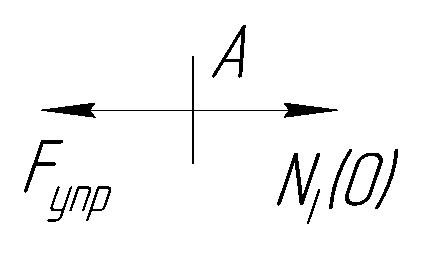
\includegraphics[width = 0.3\linewidth]{pic1.2}
            \caption{К записи условий равновесия сечения $A$}
            \label{pic1.2}
        \end{center}
    \end{figure}
    \begin{equation}
        \label{eq1.5}
        \Sigma F_x = 0
    \end{equation}
    \begin{equation}
        \label{eq1.6}
        F_{\t{упр}} = N_{I} (0)
    \end{equation}
    \begin{equation}
        \label{eq1.7}
        c u_{I} (0) = EFu_{I}' (0)
    \end{equation}
    \item Сечение $B$:
    \begin{figure}[H]
        \begin{center}
            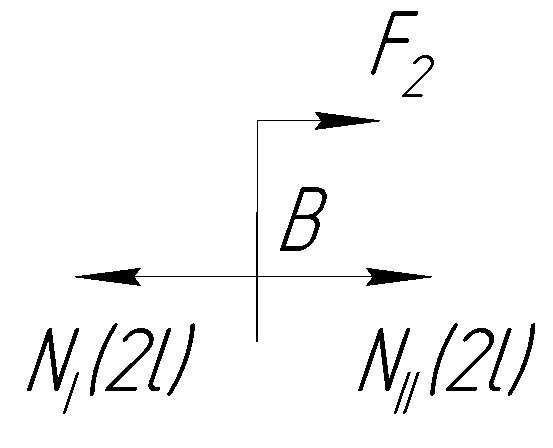
\includegraphics[width = 0.3\linewidth]{pic1.3}
            \caption{К записи условий равновесия сечения $B$}
            \label{pic1.3}
        \end{center}
    \end{figure}
    \begin{equation}
        \label{eq1.8}
        \Sigma F_x = 0
    \end{equation}
    \begin{equation}
        \label{eq1.9}
        N_{I} (2l) = F_2 + N_{II} (2l)
    \end{equation}
    \begin{equation}
        \label{eq1.9.1}
        EFu_{I}' (2l) = F_2 + EFu_{II}' (2l)
    \end{equation}
    \item Сечение $C$:
    \begin{figure}[H]
        \begin{center}
            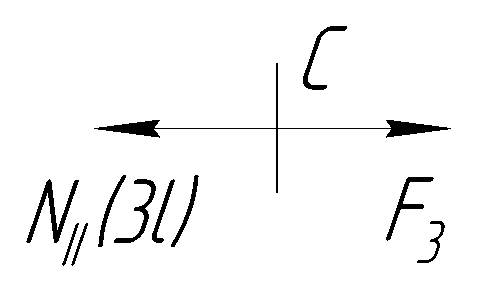
\includegraphics[width = 0.3\linewidth]{pic1.4}
            \caption{К записи условия равновесия сечения $C$}
            \label{pic1.4}
        \end{center}
    \end{figure}
    \begin{equation}
        \label{eq1.10}
        \Sigma F_x = 0
    \end{equation}
    \begin{equation}
        \label{eq1.11}
        N_{II} (3l) = F_3
    \end{equation}
    \begin{equation}
        \label{eq1.12}
        EFu_{II}' (3l) = F_3
    \end{equation}
\end{enumerate}

После нагружения в новом состоянии равновесия выполняется условие неразрывности перемещений, т.е.:
\begin{equation}
    \label{eq1.13}
    u_{I} (2l) = u_{II} (2l)
\end{equation}

Получим следующие результаты формулировки краевой задачи:
\begin{equation}
    \label{eq1.14}
    \begin{cases}
        EFu_{I}'' (x) + q = 0
        \\
        EFu_{II}'' (x) = 0
        \\
        c u_{I} (0) = EFu_{I}' (0)
        \\
        EFu_{I}' (2l) = F_2 + EFu_{II}' (2l)
        \\
        EFu_{II}' (3l) = F_3
        \\
        u_{I} (2l) = u_{II} (2l)
    \end{cases}
\end{equation}

\section{Построение точного решения краевой задачи}

Проинтегрируем дифференциальные уравнения равновесия (\ref{eq1.2}) и (\ref{eq1.3}):
\begin{enumerate}
    \item Участок $AB$:
    \begin{equation}
        \label{2.1}
        u_{I}'' (x) = - \frac{q}{EF}
    \end{equation}
    \begin{equation}
        \label{eq2.2}
        u_{I}' (x) = - \frac{qx}{EF} + C_1
    \end{equation}
    \begin{equation}
        \label{eq2.3}
        u_{I} (x) = - \frac{qx^2}{2EF} + C_1 x + C_2
    \end{equation}
    \item Участок $BC$:
    \begin{equation}
        \label{eq2.4}
        u_{II}'' (x) = 0
    \end{equation}
    \begin{equation}
        \label{eq2.5}
        u_{II}' (x) = C_3
    \end{equation}
    \begin{equation}
        \label{eq2.6}
        u_{II} (x) = C_3 x + C_4
    \end{equation}
\end{enumerate}

Подставим полученные выражения в уравнения 3-6 системы (\ref{eq1.14}):
\begin{equation}
    \label{eq2.7}
    \begin{cases}
        c \cdot C_2 = EF \cdot C_1
        \\
        \displaystyle EF \cdot (- \frac{2ql}{EF} + C_1) = F_2 + EF \cdot C_3
        \\
        EF \cdot C_3 = F_3
        \\
        \displaystyle - \frac{2ql^2}{EF} + 2 C_1 l + C_2 = 2 C_3 l + C_4
    \end{cases}
\end{equation}

Найдем константы интегрирования:
\begin{equation}
    \label{eq2.8}
    C_3 = \frac{F_3}{EF} = 0.2
\end{equation}
\begin{equation}
    \label{eq2.9}
    - 2ql + EFC_1 = F_2 + 0.2EF
\end{equation}
\begin{equation}
    \label{eq2.10}
    C_1 = \frac{F_2 + 2ql}{EF} + 0.2 = 0.5 + 2 + 0.2 = 2.7
\end{equation}
\begin{equation}
    \label{eq2.11}
    C_2 = \frac{EFC_1}{c} = \frac{C_1 l}{7} = 0.386l
\end{equation}
\begin{equation}
    \label{eq2.12}
    C_4 = - \frac{2ql^2}{EF} + 2(C_1 - C_3)l + C_2 = - 2l + 2 \cdot 2.5 l + 0.386l = 3.386l
\end{equation}

Получим итоговые функции перемещения:
\begin{equation}
    \label{eq2.13}
    \begin{cases}
        \displaystyle u_{I} (x) =  - \frac{x^2}{2l} + 2.7x + 0.386l, \; 0 \leq x \leq 2l
        \\[10pt]
        \displaystyle u_{II} (x) = 0.2x + 3.386l, \; 2l \leq x \leq 3l
    \end{cases}
\end{equation}

\begin{figure}[H]
    \begin{center}
        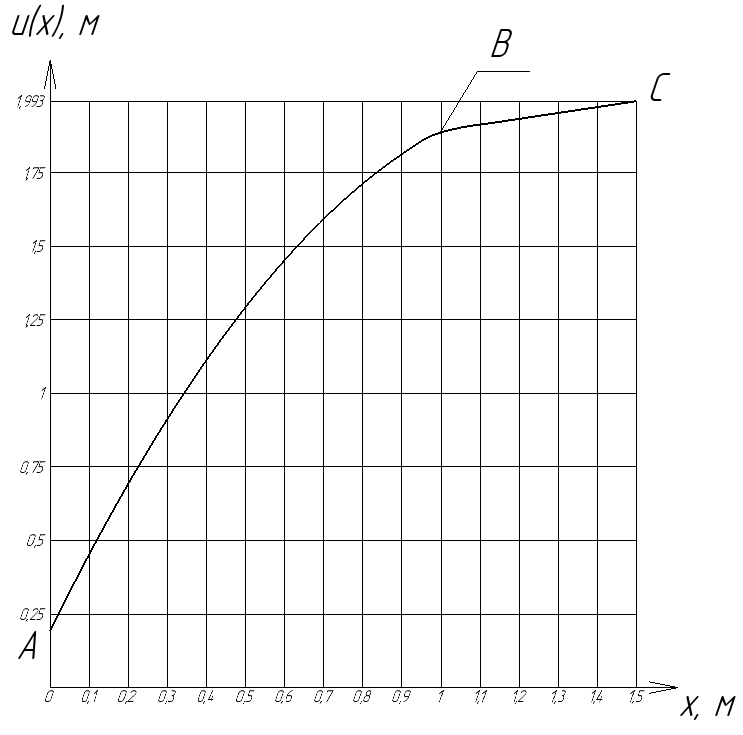
\includegraphics[width = 0.7\linewidth]{pic2.1}
        \caption{График перемещений}
        \label{pic2.1}
    \end{center}
\end{figure}

Получим функции нормальной силы $N$:
\begin{equation}
    \label{eq2.14}
    N = EFu'(x)
\end{equation}
\begin{equation}
    \label{eq2.15}
    \begin{cases}
        \displaystyle u_{I}'(x) = - \frac{x}{l} + 2.7
        \\
        \displaystyle u_{II}'(x) = 0.2
    \end{cases}
\end{equation}
\begin{equation}
    \label{eq2.16}
    \begin{cases}
        \displaystyle N_{I}(x) = (- \frac{x}{l} + 2.7) EF, \; 0 \leq x \leq 2l
        \\
        N_{II}(x) = 0.2EF, \; 2l \leq x \leq 3l
    \end{cases}
\end{equation}
\begin{figure}[H]
    \begin{center}
        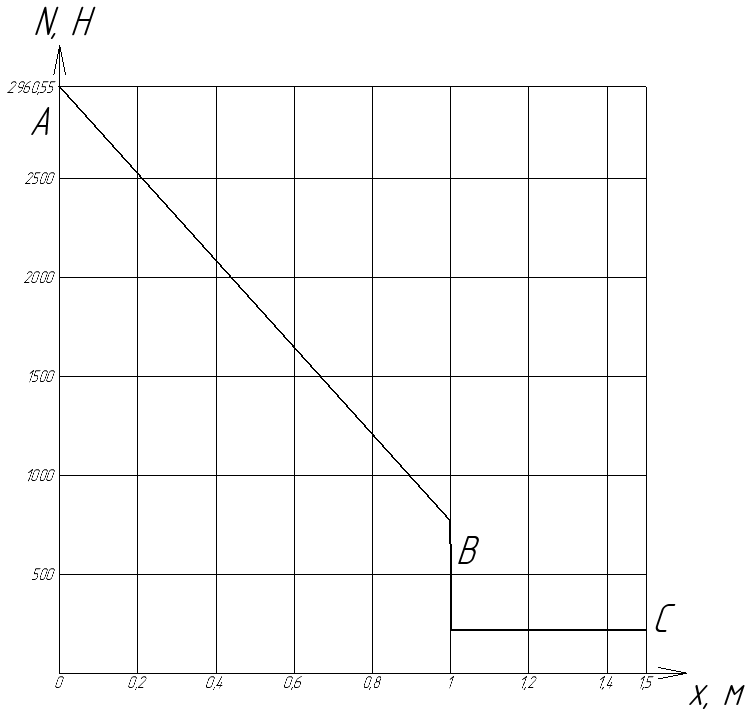
\includegraphics[width = 0.7\linewidth]{pic2.2}
        \caption{График нормальной силы $N$}
        \label{pic2.2}
    \end{center}
\end{figure}

Получим функции нормальных напряжений $\sigma (x)$:
\begin{equation}
    \label{eq2.17}
    \sigma (x) = \frac{N(x)}{F}
\end{equation}
\begin{equation}
    \label{eq2.18}
    \begin{cases}
        \displaystyle \sigma_{I} (x) = (- \frac{x}{l} + 2.7) E, \; 0 \leq x \leq 2l
        \\
        \displaystyle \sigma_{II} (x) = 0.2E, \; 2l \leq x \leq 3l
    \end{cases}
\end{equation}
\begin{figure}[H]
    \begin{center}
        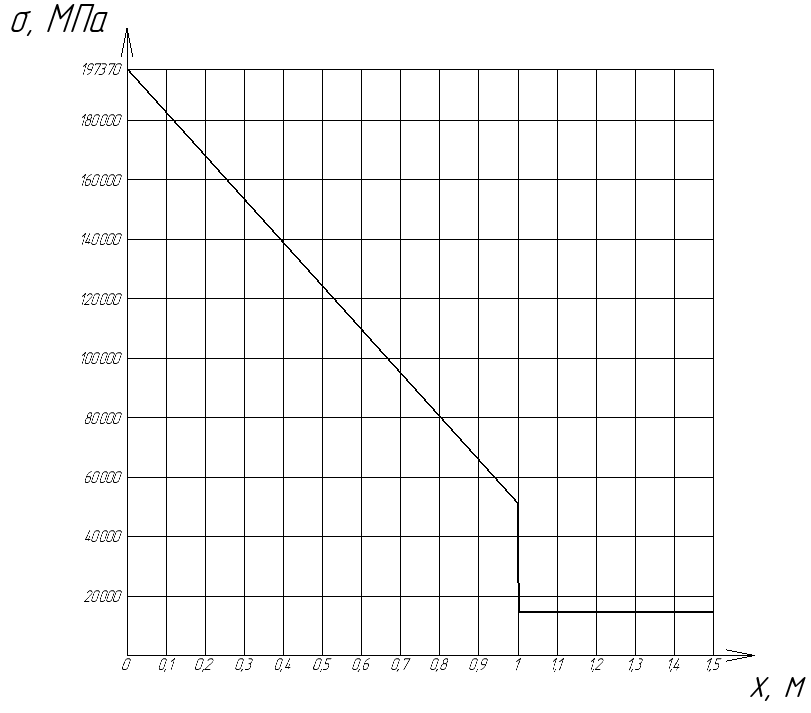
\includegraphics[width = 0.7\linewidth]{pic2.3}
        \caption{График нормальных напряжений}
        \label{pic2.3}
    \end{center}
\end{figure}

\section{Преобразование краевой задачи в вариационный принцип}

Запишем невязку дифференциального уравнения краевой задачи (\ref{eq1.14}):
\begin{itemize}
    \item для участка $AB$:
    \begin{equation}
        \label{eq3.1}
        L[u_I] = EFu_I''(x) + q
    \end{equation}
    \item для участка $BC$:
    \begin{equation}
        \label{eq3.2}
        L[u_{II}] = EFu_{II}''(x)
    \end{equation}
\end{itemize}

В операторной форме невязка выглядит следующим образом:
\begin{equation}
    \label{eq3.3}
    L[u] = Au - f
\end{equation}
где $\displaystyle A = EF\frac{d^2}{dx^2}$ --- дифференциальный оператор краевой задачи, $f = -q$.

Запишем условие аннулирования невязки:
\begin{equation}
    \label{eq3.4}
    \int_{0}^{L} L[u] \phi_k(x) dx = 0, \; k=1,2,3 \dots \infty
\end{equation}
где $u(x)$ имеет вид:
\begin{equation}
    \label{eq3.5}
    u(x) = \sum_{i = 1}^{\infty} \alpha_i \phi_i(x)
\end{equation}
где $\phi_i(x)$ --- базисные функции, $\alpha_i$ --- некоторые коэффициенты.

Выражение (\ref{eq3.4}) представляет собой систему уравнений
\begin{equation}
    \label{eq3.6}
    \begin{cases}
        \displaystyle \int_{0}^{L} L[u] \phi_1(x) dx = 0
        \\
        \displaystyle \int_{0}^{L} L[u] \phi_2(x) dx = 0
        \\
        \dots
        \\
        \displaystyle \int_{0}^{L} L[u] \phi_n(x) dx = 0
    \end{cases}
\end{equation}

Эти уравнения можно привести к удобному для рассмотрения виду. Для этого запишем вариацию (\ref{eq3.5}):
\begin{equation}
    \label{eq3.7}
    \delta u = \sum_{i = 1}^{\infty} \delta \alpha_i \phi_i
\end{equation}

Уравнения (\ref{eq3.6}) умножим на $\delta \alpha_i$ соответственно и сложим:
\begin{equation}
    \label{eq3.8}
    \int_{0}^{L} L[u] (\sum_{i = 0}^{\infty} \delta \alpha_i \phi_i) dx = 0
\end{equation}
\begin{equation}
    \label{eq3.9}
    \int_{0}^{L} L[u] \delta u dx = 0
\end{equation}

Запишем вариационное уравнение (\ref{eq3.9}) для нашей задачи:
\begin{equation}
    \label{eq3.10}
    \int_{0}^{2l} (EFu_I''(x) + q)\delta u_I(x) dx + \int_{2l}^{3l} EFu_{II}''(x) \delta u_{II}(x) dx = 0
\end{equation}
\begin{equation}
    \label{eq3.11}
    \int_{0}^{2l} EFu_I''(x) \delta u_I(x) dx + \int_{2l}^{3l} EFu_{II}''(x) \delta u_{II}(x) dx + \int_{0}^{2l} q \delta u(x) dx = 0
\end{equation}

Преобразуем первые 2 слагаемых:
\begin{equation}
    \label{eq3.12}
    \int_{0}^{2l} EFu_I''(x) \delta u_I(x) dx = \int_{0}^{2l} EF \delta u_I du_I' = EFu_I' \delta u_I \Big|_{0}^{2l} - \int_{0}^{2l} EFu_I' \delta u_I' dx
\end{equation}
\begin{equation}
    \label{eq3.13}
    \int_{2l}^{3l} EFu_{II}''(x) \delta u_{II}(x) dx = \int_{2l}^{3l} EF \delta u_{II} du_{II}' = EFu_{II}' \delta u_{II} \Big|_{2l}^{3l} - \int_{2l}^{3l} EFu_{II}' \delta u_{II}' dx
\end{equation}

Подставим (\ref{eq3.12}) и (\ref{eq3.13}) в (\ref{eq3.11}):
\begin{equation}
    \label{eq3.14}
    \begin{split}
        & EFu_I'(2l) \delta u_I(2l) - EFu_I'(0) \delta u_I(0) - \int_{0}^{2l} EFu_I' \delta u_I' dx + EFu_{II}'(3l) \delta u_{II}(3l) -
        \\
        & - EFu_{II}'(2l) \delta u_{II}(2l) - \int_{2l}^{3l} EFu_{II}' \delta u_{II}' dx + \int_{0}^{2l} q \delta u_I dx = 0
    \end{split}
\end{equation}

Учтем граничные условия из формулировки краевой задачи (\ref{eq1.14}) и условие $\delta u_I(2l) = \delta u_{II}(2l)$:
\begin{equation}
    \label{eq3.15}
    \begin{split}
        & F_2 \delta u_I(2l) - cu_I(0) \delta u_I(0) + F_3 \delta u_{II}(3l) -
        \\
        & - \int_{0}^{2l} EFu_I' \delta u_I' dx - \int_{2l}^{3l} EFu_{II}' \delta u_{II}' dx + \int_{0}^{2l} q \delta u_I dx = 0
    \end{split}
\end{equation}

Преобразуем (\ref{eq3.15}), используя правила варьирования:
\begin{equation}
    \label{eq3.16}
    \begin{split}
        & \delta \Big[ \frac{1}{2} \int_{0}^{2l} EF{u_I'}^2 dx + \frac{1}{2} \int_{2l}^{3l} EF{u_{II}'}^2 dx - \int_{0}^{2l} qu_I dx + \frac{1}{2} cu_I^2(0) - F_2 u_I(2l) -
        \\
        & - F_3 u_{II}(3l) \Big] = 0
    \end{split}
\end{equation}

Тогда функционал полной потенциальной энергии равен:
\begin{equation}
    \label{eq3.17}
    \begin{split}
        & \t{П} [u_I, u_{II}] = \frac{1}{2} \int_{0}^{2l} EF{u_I'}^2 dx + \frac{1}{2} \int_{2l}^{3l} EF{u_{II}'}^2 dx - \int_{0}^{2l} qu_I dx + \frac{1}{2} cu_I^2(0) - F_2 u_I(2l) -
        \\
        & - F_3 u_{II}(3l)
    \end{split}
\end{equation}
и выражение (\ref{eq3.16}) можно переписать в виде:
\begin{equation}
    \label{eq3.18}
    \delta \t{П} = 0
\end{equation}

Выражение (\ref{eq3.18}) является условием стационарности функционала полной потенциальной энергии, которое согласно принципу Лагранжа выполняется на точном решении краевой задачи.

\section{Получение решения энергетическим методом на линейной аппроксимации поля перемещений}

Аппроксимируем поле перемещений кусочно-линейными функциями:
\begin{itemize}
    \item Первый участок (первая половина $AB$)
    \begin{equation}
        \label{eq4.1}
        u_I(x) = u_0 + \frac{u_1 - u_0}{l}x, \;\;\; 0 \leq x \leq l
    \end{equation}
    где $u_0 = u(0)$, $u_1 = u(l)$.
    \item Второй участок (вторая половина $AB$) \\
    Введем новую систему координат $O \tilde{x}$ с началом в точке $x = l$. Тогда
    \begin{equation}
        \label{eq4.2}
        u_{II}(\tilde{x}) = u_1 + \frac{u_2 - u_1}{l} \tilde{x}, \;\;\; 0 \leq \tilde{x} \leq l
    \end{equation}
    где $u_2 = u(2l)$.
    \item Третий участок ($BC$) \\
    Введем новую систему координат $O \hat{x}$ с началом в точке $x = 2l$. Тогда
    \begin{equation}
        \label{eq4.2.1}
        u_{III}(x) = u_2 + \frac{u_3 - u_2}{l} \hat{x}, \;\;\; 0 \leq \hat{x} \leq l
    \end{equation}
    где $u_3 = u(3l)$
\end{itemize}

Получим следующий функционал:
\begin{equation}
    \label{eq4.3}
    \begin{split}
        & \t{П} [u_I, u_{II}, u_{III}] = \frac{1}{2} \int_{0}^{l} EF{u_I'}^2(x) dx + \frac{1}{2} \int_{0}^{l} EF{u_{II}'}^2(\tilde{x}) d\tilde{x} + \frac{1}{2} \int_{0}^{l} EF{u_{III}'}^2(\tilde{x}) d\tilde{x} - 
        \\
        & - \int_{0}^{l} qu_I(x)dx - \int_{0}^{l} qu_{II}(\tilde{x})dx + \frac{1}{2}cu_0^2 - F_2 u_2 - F_3 u_3
    \end{split}
\end{equation}

Найдем производные функций перемещения:
\begin{equation}
    \label{eq4.4}
    u_I'(x) = \frac{u_1 - u_0}{l}
\end{equation}
\begin{equation}
    \label{eq4.5}
    u_{II}'(\tilde{x}) = \frac{u_2 - u_1}{l}
\end{equation}
\begin{equation}
    \label{eq4.5.1}
    u_{III}'(\hat{x}) = \frac{u_3 - u_2}{l}
\end{equation}

Подставим (\ref{eq4.4}) и (\ref{eq4.5}) в функционал (\ref{eq4.3}):
\begin{equation}
    \label{eq4.6}
    \begin{split}
        & \t{П}[u_0, u_1, u_2, u_3] = \frac{1}{2} EF \left[ \left( \frac{u_1 - u_0}{l} \right)^2 \cdot l + \left( \frac{u_2 - u_1}{l} \right)^2 \cdot l + \left( \frac{u_3 - u_2}{l} \right)^2 \cdot l \right] - 
        \\
        & - q \left( (u_0 + u_1)l + \frac{u_2 - u_0}{l} \frac{l^2}{2} \right) + \frac{1}{2}cu_0^2 - F_2u_2 - F_3u_3
    \end{split}
\end{equation}

Запишем условие стационарности функционала (\ref{eq4.6}):
\begin{equation}
    \label{eq4.7}
    \begin{cases}
        \displaystyle \frac{\partial \t{П}}{\partial u_0} = 0
        \\[10pt]
        \displaystyle \frac{\partial \t{П}}{\partial u_1} = 0
        \\[10pt]
        \displaystyle \frac{\partial \t{П}}{\partial u_2} = 0
        \\[10pt]
        \displaystyle \frac{\partial \t{П}}{\partial u_3} = 0
    \end{cases}
\end{equation}

Распишем выражения (\ref{eq4.7}):
\begin{equation}
    \label{eq4.8}
    \frac{(u_1 - u_0)EF}{l} = u_0c - \frac{ql}{2}
\end{equation}
\begin{equation}
    \label{eq4.8.1}
    \frac{(2u_1 - u_0 - u_2)EF}{l} = ql
\end{equation}
\begin{equation}
    \label{eq4.9}
    \frac{(4u_2 - 2u_1 - 2u_3)EF}{2l} = F_2 + \frac{ql}{2}
\end{equation}
\begin{equation}
    \label{eq4.10}
    \frac{(u_3 - u_2)EF}{l} = F_3
\end{equation}

Из (\ref{eq4.8}) выразим $u_1$:
\begin{equation}
    \label{eq4.11}
    u_1 = u_0 \left( 1 + \frac{cl}{EF} \right) - \frac{ql^2}{2EF}
\end{equation}

Подставим (\ref{eq4.11}) в (\ref{eq4.8.1}) и выразим $u_2$:
\begin{equation}
    \label{eq4.12}
    u_2 = u_0 \left( 1 + \frac{2cl}{EF} \right) - \frac{2ql^2}{EF}
\end{equation}

Подставим (\ref{eq4.12}) и (\ref{eq4.11}) в (\ref{eq4.9}) и выразим $u_3$:
\begin{equation}
    \label{eq4.13}
    u_3 = u_0 \left( 1 + \frac{3cl}{EF} \right) - \frac{4ql^2 + F_2l}{EF}
\end{equation}

Подставим (\ref{eq4.13}) в (\ref{eq4.12}) в (\ref{eq4.10}) и найдем $u_0$:
\begin{equation}
    \label{eq4.14}
    u_0 = \frac{2ql + F_2 + F_3}{c}
\end{equation}

Найдем оставшиеся коэффициенты:
\begin{equation}
    \label{eq4.14.1}
    u_1 = \frac{(3ql + 2F_2 + 2F_3)l}{2EF} + \frac{2ql + F_2 + F_3}{c}
\end{equation}
\begin{equation}
    \label{eq4.15}
    u_2 = \frac{(2ql + 2F_2 + 2F_3)l}{EF} + \frac{2ql + F_2 + F_3}{c}
\end{equation}
\begin{equation}
    \label{eq4.15.1}
    u_3 = \frac{(2ql + 2F_2 + 3F_3)l}{EF} + \frac{2ql + F_2 + F_3}{c}
\end{equation}

Подставим исходные данные (\ref{eq0.1}) в полученные выражения:
\begin{equation}
    \label{eq4.16}
    u_0 = 0.386 l
\end{equation}
\begin{equation}
    \label{eq4.17}
    u_1 = 2.586 l
\end{equation}
\begin{equation}
    \label{eq4.18}
    u_2 = 3.786 l
\end{equation}
\begin{equation}
    \label{eq4.18.1}
    u_3 = 3.986 l
\end{equation}

Получим итоговые выражения для функций перемещений:
\begin{equation}
    \label{eq4.19}
    u_I(x) = 2.2x + 0.386l, \;\;\; 0 \leq x \leq 2l
\end{equation}
\begin{equation}
    \label{eq4.20}
    u_{II}(\tilde{x}) = 1.2 \tilde{x} + 2.586 l, \;\;\; 0 \leq \tilde{x} \leq l
\end{equation}
или
\begin{equation}
    \label{eq4.21}
    u_{II}(x) = 1.2x + 1.386 l, \;\;\; l \leq x \leq 2l
\end{equation}\
\begin{equation}
    \label{eq4.21.1}
    u_{III}(\hat{x}) = 0.2 \hat{x} + 3.786 l, \;\;\; 0 \leq \hat{x} \leq l
\end{equation}
или
\begin{equation}
    \label{eq4.21.2}
    u_{III}(x) = 0.2 x + 3.386 l, \;\;\; 2l \leq x \leq 3l
\end{equation}

\begin{figure}[H]
    \begin{center}
        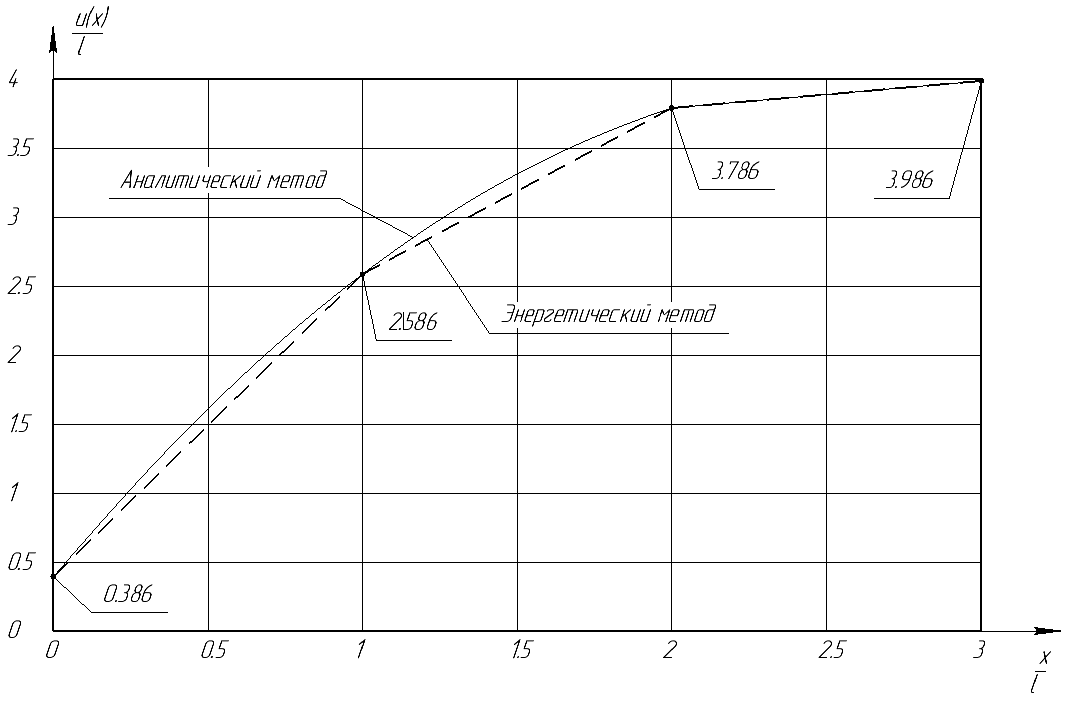
\includegraphics[width = 0.7\linewidth]{pic4.1.PNG}
        \caption{График перемещений, полученных энергетическим и аналитическим методом}
        \label{pic4.1}
    \end{center}
\end{figure}

Найдем внутренние усилия:
\begin{equation}
    \label{eq4.22}
    N(x) = EFu'(x)
\end{equation}
\begin{equation}
    \label{eq4.23}
    N_I(x) = 2.2 EF, \;\;\; 0 \leq x \leq l
\end{equation}
\begin{equation}
    \label{eq4.24}
    N_{II}(x) = 1.2EF, \;\;\; l \leq x \leq 2l
\end{equation}
\begin{equation}
    \label{eq4.24.1}
    N_{III}(x) = 0.2 EF, \;\;\; 2l \leq x \leq 3l
\end{equation}

\begin{figure}[H]
    \begin{center}
        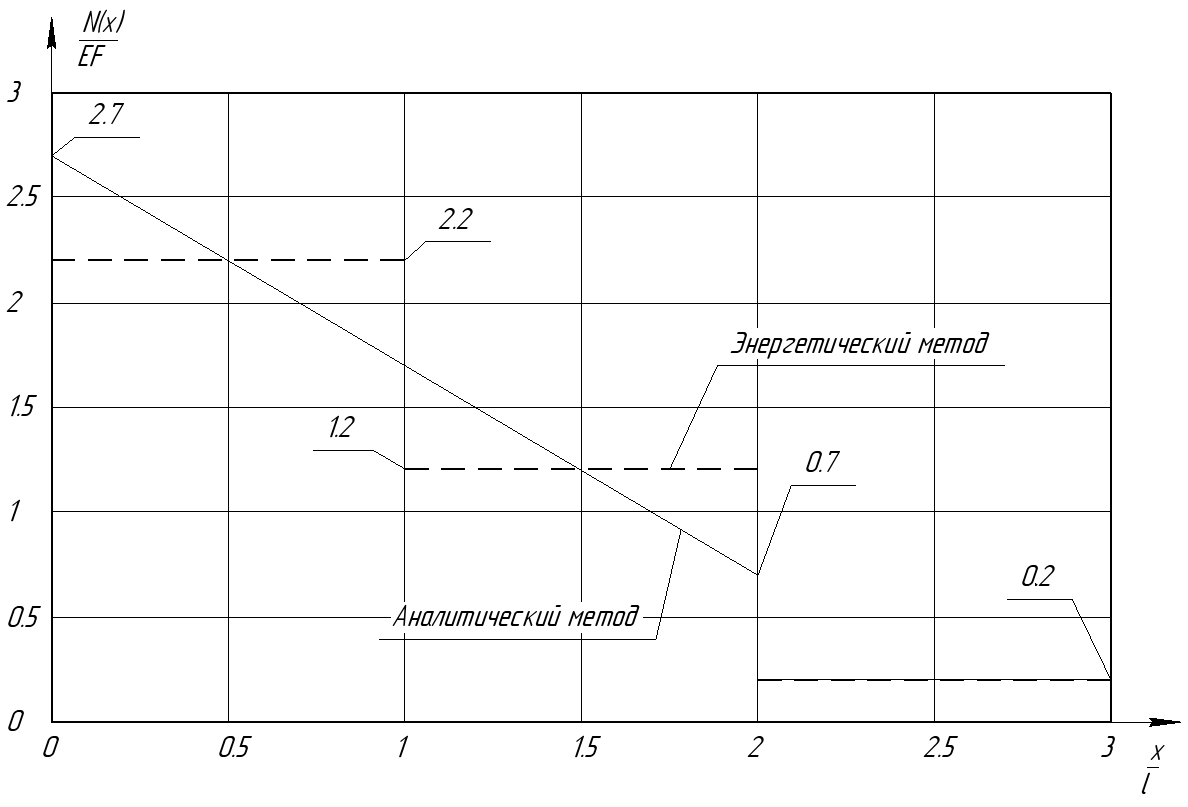
\includegraphics[width = 0.7\linewidth]{pic4.2.PNG}
        \caption{График нормальной силы, полученной энергетическим и аналитическим методами}
        \label{pic4.2}
    \end{center}
\end{figure}

Найдем нормальные напряжения:
\begin{equation}
    \label{eq4.25}
    \sigma(x) = \frac{N(x)}{F}
\end{equation}
\begin{equation}
    \label{eq4.26}
    \sigma_I(x) = 2.2E, \;\;\; 0 \leq x \leq l
\end{equation}
\begin{equation}
    \label{eq4.27}
    \sigma_{II}(x) = 1.2E, \;\;\; l \leq x \leq 2l
\end{equation}
\begin{equation}
    \label{eq4.27.1}
    \sigma_{III}(x) = 0.2E, \;\;\; 2l \leq x \leq 3l
\end{equation}

\begin{figure}[H]
    \begin{center}
        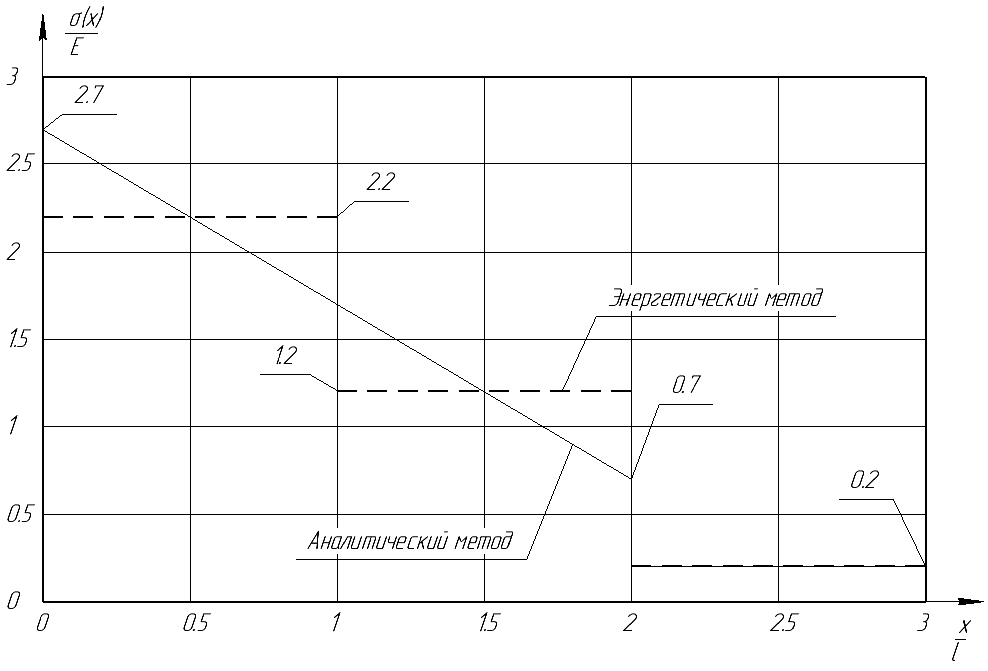
\includegraphics[width = 0.7\linewidth]{pic4.3.PNG}
        \caption{График нормальных напряжений, полученных энергетическим и аналитическим методами}
        \label{pic4.3}
    \end{center}
\end{figure}

\section{Оценка погрешности по энергии между точным и приближенным решением}

Запишем выражение для функционала полной потенциальной энергии на приближенном решении:
\begin{equation}
    \label{eq5.1}
    \begin{split}
        & \t{П}[u_0, u_1, u_2, u_3] = \frac{1}{2} EF \left[ \left( \frac{u_1 - u_0}{l} \right)^2 \cdot l + \left( \frac{u_2 - u_1}{l} \right)^2 \cdot l + \left( \frac{u_3 - u_2}{l} \right)^2 \cdot l \right] - 
        \\
        & - q \left( (u_0 + u_1)l + \frac{u_2 - u_0}{l} \frac{l^2}{2} \right) + \frac{1}{2}cu_0^2 - F_2u_2 - F_3u_3
    \end{split}
\end{equation}

Подставим в (\ref{eq5.1}) значения (\ref{eq4.16}), (\ref{eq4.17}), (\ref{eq4.18}) и (\ref{eq0.1}) и получим:
\begin{equation}
    \label{eq5.2}
    \t{П}_\t{э} = \t{П}[u_0, u_1, u_2, u_3] = -3.68071 EFl
\end{equation}

Запишем выражение для функционала полной функциональной энергии на точном решении, используя выражения (\ref{eq2.13}):
\begin{equation}
    \label{eq5.3}
    \begin{split}
        & \t{П} [u_I, u_{II}] = \frac{1}{2} \int_{0}^{2l} EF{u_I'}^2 dx + \frac{1}{2} \int_{2l}^{3l} EF{u_{II}'}^2 dx - \int_{0}^{2l} qu_I dx + \frac{1}{2} cu_I^2(0) - F_2 u_I(2l) -
        \\
        & - F_3 u_{II}(3l)
    \end{split}
\end{equation}
\begin{equation}
    \label{eq5.4}
    \t{П}_\t{а} = \t{П}[u_I, u_{II}] = -3.76405 EFl
\end{equation}

Расчитаем погрешность:
\begin{equation}
    \label{eq5.5}
    \Delta = \Big| \frac{\t{П}_\t{э} - \t{П}_\t{а}}{\t{П}_\t{а}} \Big| \cdot 100 \% = 2.214 \%
\end{equation}